%%%%%%%%%%%%%%%%%%%%%%%%%%%%%%%%%%%%%%%%%%%%%%%%%%%
%% LaTeX book template                           %%
%% Author:  Amber Jain (http://amberj.devio.us/) %%
%% License: ISC license                          %%
%%%%%%%%%%%%%%%%%%%%%%%%%%%%%%%%%%%%%%%%%%%%%%%%%%%

\documentclass[a4paper,11pt,oneside]{book}
\usepackage{modulestyle}

%%%%%%%%%%%%%%%%%%%%%%%%%%%%%%%%%%%%%%%%%%%%%%%%%%%%%%%%%
% Source: http://en.wikibooks.org/wiki/LaTeX/Hyperlinks %
%%%%%%%%%%%%%%%%%%%%%%%%%%%%%%%%%%%%%%%%%%%%%%%%%%%%%%%%%

%%%%%%%%%%%%%%%%%%%%%%%%%%%%%%%%%%%%%%%%%%%%%%%%%%%%%%%%%%%%%%%%%%%%%%%%%%%%%%%%
% 'dedication' environment: To add a dedication paragraph at the start of book %
% Source: http://www.tug.org/pipermail/texhax/2010-June/015184.html            %
%%%%%%%%%%%%%%%%%%%%%%%%%%%%%%%%%%%%%%%%%%%%%%%%%%%%%%%%%%%%%%%%%%%%%%%%%%%%%%%%
\newenvironment{dedication}
{
   \cleardoublepage
   \thispagestyle{empty}
   \vspace*{\stretch{1}}
   \hfill\begin{minipage}[t]{0.66\textwidth}
   \raggedright
}
{
   \end{minipage}
   \vspace*{\stretch{3}}
   \clearpage
}

%%%%%%%%%%%%%%%%%%%%%%%%%%%%%%%%%%%%%%%%%%%%%%%%
% Chapter quote at the start of chapter        %
% Source: http://tex.stackexchange.com/a/53380 %
%%%%%%%%%%%%%%%%%%%%%%%%%%%%%%%%%%%%%%%%%%%%%%%%
\makeatletter
\renewcommand{\@chapapp}{}% Not necessary...
\newenvironment{chapquote}[2][2em]
  {\setlength{\@tempdima}{#1}%
   \def\chapquote@author{#2}%
   \parshape 1 \@tempdima \dimexpr\textwidth-2\@tempdima\relax%
   \itshape}
  {\par\normalfont\hfill--\ \chapquote@author\hspace*{\@tempdima}\par\bigskip}
\makeatother

%%%%%%%%%%%%%%%%%%%%%%%%%%%%%%%%%%%%%%%%%%%%%%%%%%%
% First page of book which contains 'stuff' like: %
%  - Book title, subtitle                         %
%  - Book author name                             %
%%%%%%%%%%%%%%%%%%%%%%%%%%%%%%%%%%%%%%%%%%%%%%%%%%%

\newcommand{\BookTitle}{Programming Fundamentals}
\newcommand{\BookTitleFootnote}{A course in the Bachelor of Technical Vocational Teacher Education (BTVTED) Major in Computer System Servicing.}

\newcommand{\BookSubtitle}{A Study Guide for Students of Sorsogon State University - Bulan Campus}
\newcommand{\BookSubtitleFootnote}{This book is a study guide for students of
Sorsogon State University - Bulan Campus taking up the course Programming Fundamentals.}

\newcommand{\BookAuthorFirstName}{Jarrian Vince}
\newcommand{\BookAuthorLastName}{Gojar}
\newcommand{\BookAuthorName}{Jarrian Vince G. Gojar}
\newcommand{\BookAuthorURL}{https://github.com/godkingjay}

% Book's title and subtitle
\title{\Huge \textbf{\BookTitle}  \footnote{\BookTitleFootnote} \\
\huge \BookSubtitle \footnote{\BookSubtitleFootnote}}

% Author
\author{\textsc{\BookAuthorName}\thanks{\url{\BookAuthorURL}}}

\begin{document}

\frontmatter
\maketitle

%%%%%%%%%%%%%%%%%%%%%%%%%%%%%%%%%%%%%%%%%%%%%%%%%%%%%%%%%%%%%%%
% Add a dedication paragraph to dedicate your book to someone %
%%%%%%%%%%%%%%%%%%%%%%%%%%%%%%%%%%%%%%%%%%%%%%%%%%%%%%%%%%%%%%%
\begin{dedication}
    Sorsogon State University - Bulan Campus
\end{dedication}

%%%%%%%%%%%%%%%%%%%%%%%%%%%%%%%%%%%%%%%%%%%%%%%%%%%%%%%%%%%%%%%%%%%%%%%%
% Auto-generated table of contents, list of figures and list of tables %
%%%%%%%%%%%%%%%%%%%%%%%%%%%%%%%%%%%%%%%%%%%%%%%%%%%%%%%%%%%%%%%%%%%%%%%%
\tableofcontents
\listoffigures
\listoftables
\lstlistoflistings

\mainmatter

%%%%%%%%%%%
% Preface %
%%%%%%%%%%%
\chapter*{Preface}
% A Quote all about Programming Fundamentals
\begin{chapquote}{Donald Ervin Knuth}
    ``Programming is the art of telling another human being what one wants
    the computer to do.''
\end{chapquote}

\noindent \BookAuthorName \\
\noindent \url{\BookAuthorURL}

%%%%%%%%%%%%%%%%%%%%%%%%%%%%%%%%%%%%
%%%%%~ NEW CHAPTER STARTS HERE %%%%%
%%%%%%%%%%%%%%%%%%%%%%%%%%%%%%%%%%%%
\chapter{Introduction to Python}

\section{Introduction}

\textbf{Python} is a high-level, interpreted, interactive, and
object-oriented programming language. It is designed to be highly
readable, using English keywords frequently, unlike other languages
that use punctuation, and it has fewer syntactical constructions. It is
a versatile, general-purpose, and powerful programming language. It
is an excellent first language because it is concise and easy to read. Whether
you want to do web development, machine learning, or data science, Python is
the language for you.

\subsection{History of Python}

Python was developed by \textbf{Guido van Rossum} in the late 80's and early
90's at the National Research Institute for Mathematics and Computer Science in
the Netherlands. Python is derived from many other languages, including ABC,
Modula-3, C, C++, Algol-68, SmallTalk, and Unix shell and other scripting
languages.

\subsection{What is Programming Language?}

A programming language is a formal language comprising a set of instructions
that produce various kinds of output. Programming languages are used in
computer programming to implement algorithms. A computer only understands
machine code, which is a series of binary numbers. Programming languages allow
humans to write code that can be understood by computers. Python in particular
is an interpreted language, which means that the code is executed line by line.

\section{Environment Setup}

In software development, an \textbf{integrated development environment (IDE)}
is a software application that provides comprehensive facilities to computer
programmers for software development. An IDE normally consists of a source code
editor, build automation tools, and a debugger. Other than the IDE, it is also
important to have the programming language installed on your computer.

\subsection{How to Download and Install Python on Windows}

To download and install Python on Windows, follow these steps:

\begin{enumerate}
    \item Open a web browser and go to the official Python website at
          \url{https://www.python.org/downloads/}.
    \item Click on the latest version of Python to download the installer.
    \item Run the installer and follow the installation wizard.
    \item Make sure to check the box that says ``Add Python to PATH''.
    \item Click on the ``Install Now'' button to install Python on your computer.

          \begin{figure}[!h]
              \centering
              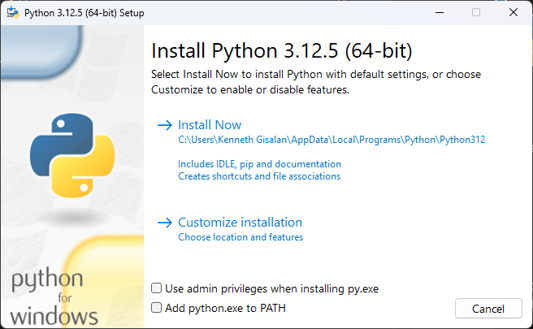
\includegraphics[width=0.8\textwidth]{./assets/setup/python-install.png}
              \caption{Python Installation Wizard}
              \label{fig:python-install}
          \end{figure}

    \item Once the installation is complete, you can verify the installation by opening a
          command prompt and typing \texttt{python --version}.

          \begin{figure}[!h]
              \centering
              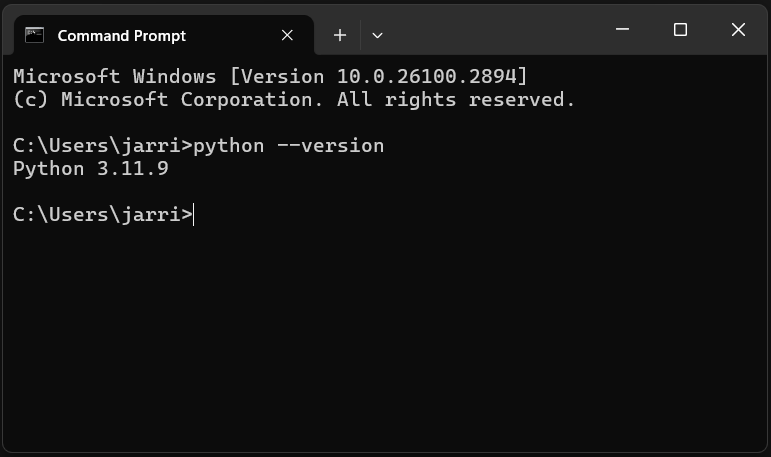
\includegraphics[width=0.8\textwidth]{./assets/setup/python-check.png}
              \caption{Python Installation Verification}
              \label{fig:python-check}
          \end{figure}
\end{enumerate}

\subsection{How to Download PyCharm IDE on Windows}

To download and install PyCharm IDE on Windows, follow these steps:

\begin{enumerate}
    \item Open a web browser and go to the official PyCharm website at
          \url{https://www.jetbrains.com/pycharm/download/}.
    \item Click on the ``Download'' button to download the installer.

          \begin{figure}[!h]
              \centering
              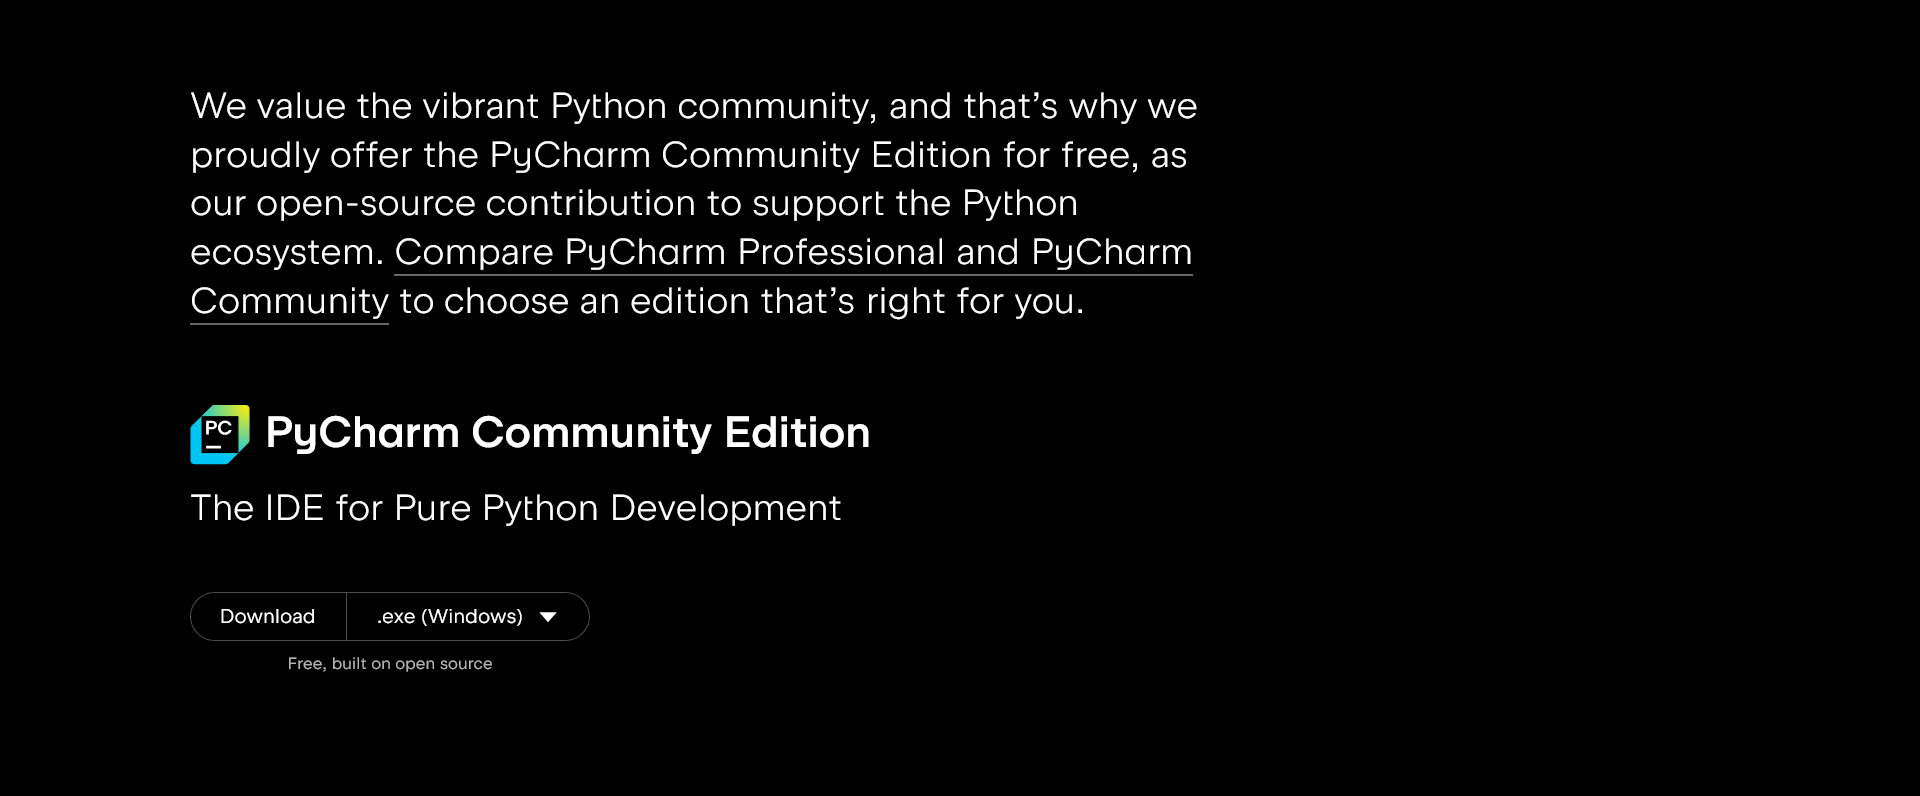
\includegraphics[width=0.8\textwidth]{./assets/setup/pycharm-community.png}
              \caption{PyCharm Community Edition Download}
              \label{fig:pycharm-community}
          \end{figure}

    \item Run the installer and follow the installation wizard.
    \item Make sure to check the box that says ``Create associations''.
    \item Click on the ``Install'' button to install PyCharm on your computer.

          \begin{figure}[!h]
              \centering
              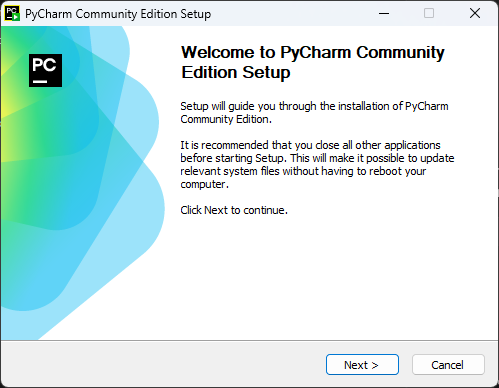
\includegraphics[width=0.8\textwidth]{./assets/setup/pycharm-install.png}
              \caption{PyCharm Community Edition Installation Wizard}
              \label{fig:pycharm-install}
          \end{figure}

    \item Once the installation is complete, you can launch PyCharm by clicking on the
          desktop shortcut or searching for it in the Start menu.
\end{enumerate}

\section{First Python Program}

In Python, the \texttt{print()} function is used to display output on the
screen. To write your first Python program, follow these steps:

\begin{enumerate}
    \item Open PyCharm IDE on your computer.
    \item Click on the ``Create New Project'' button to create a new project.
    \item Enter a name for your project and click on the ``Create'' button.
    \item Right-click on the project folder in the Project view and select ``New''
          $\rightarrow$ ``Python File''.
    \item Enter a name for your Python file and click on the ``OK'' button.
    \item Type the following code in the Python file:

          \begin{lstlisting}[language=Python, caption={Hello, World! Program}, label={lst:hello-world}]
    print("Hello, World!")
    \end{lstlisting}

    \item Click on the ``Run'' button to run the program.
    \item You should see the output ``Hello, World!'' displayed in the Run window.
\end{enumerate}

\section{Basic Syntax}

In Python, the syntax refers to the rules that define the combinations of
symbols that are considered to be correctly structured programs in the
language. The Python syntax is simple and easy to learn. It is based on
indentation and does not require the use of curly braces or semicolons. It can
also be easily understood by beginners as it is very similarly structured to
the English language.

\subsection{Variables}

A variable is a name that refers to a value. In Python, variables are created
when you assign a value to them. You can assign a value to a variable using the
assignment operator \texttt{=}.

\begin{lstlisting}[language=Python, caption={Variable Assignment}, label={lst:variables}]
x = 5
y = "Hello, World!"

print(x)
print(y)
\end{lstlisting}

Code \ref{lst:variables} shows how to assign values to variables in Python. In
this example, the variable \texttt{x} is assigned the value 5, and the variable
\texttt{y} is assigned the value ``Hello, World!''.

\newpage

\noindent\textbf{Exercises}
\begin{lstlisting}[numbers=none]
1. Create a variable called `name` and assign the value to your name.
2. Create a variable called `age` and assign the value to your age.
3. Create a variable called `address` and assign the value to your address.
4. Print the values of the variables `name`, `age`, and `address`.
\end{lstlisting}

\subsection{Python Identifiers}

An identifier is a name given to entities like class, functions, variables,
etc. It helps to differentiate one entity from another. In Python, an
identifier is a name used to identify a variable, function, class, module, or
other object. An identifier must start with a letter or an underscore (\_),
followed by letters, digits, or underscores.

\begin{lstlisting}[language=Python, caption={Valid and Invalid Identifiers}, label={lst:identifiers}]
# Valid Identifiers
my_variable = 5
myVariable = 10
_my_variable = 15

# Invalid Identifiers
1variable = 20
my-variable = 25
my variable = 30
\end{lstlisting}

Code \ref{lst:identifiers} shows examples of valid and invalid identifiers in
Python. In this example, the variables \texttt{my\_variable},
\texttt{myVariable}, and \texttt{\_my\_variable} are valid identifiers, while
the variables \texttt{1variable}, \texttt{my-variable}, and \texttt{my
    variable} are invalid identifiers.

\noindent\textbf{Exercises}
\begin{lstlisting}[numbers=none]
1. Create a variable called `first_name` and assign the value to your first name.
2. Create a variable called `last_name` and assign the value to your last name.
3. Create a variable called `full_name` and assign the value of concatenating `first_name` and `last_name`.
4. Print the value of the variable `full_name`.
\end{lstlisting}

\subsection{Reserved Words}

Python has a set of reserved words that cannot be used as identifiers. These
reserved words are used by the Python interpreter to recognize the structure of
the program. Some of the reserved words in Python include:

\begin{multicols}{4}
    \begin{itemize}
        \item \texttt{False}
        \item \texttt{None}
        \item \texttt{True}
        \item \texttt{and}
        \item \texttt{as}
        \item \texttt{assert}
        \item \texttt{break}
        \item \texttt{class}
        \item \texttt{continue}
        \item \texttt{def}
        \item \texttt{del}
        \item \texttt{elif}
        \item \texttt{else}
        \item \texttt{except}
        \item \texttt{exec}
        \item \texttt{finally}
        \item \texttt{for}
        \item \texttt{from}
        \item \texttt{global}
        \item \texttt{if}
        \item \texttt{import}
        \item \texttt{in}
        \item \texttt{is}
        \item \texttt{lambda}
        \item \texttt{nonlocal}
        \item \texttt{not}
        \item \texttt{or}
        \item \texttt{pass}
        \item \texttt{print}
        \item \texttt{raise}
        \item \texttt{return}
        \item \texttt{try}
        \item \texttt{while}
        \item \texttt{with}
        \item \texttt{yield}
    \end{itemize}
\end{multicols}

These reserved words cannot be used as identifiers in Python. They cannot be
used as variable names, function names, or any other identifier names.

\subsection{Quotation in Python}

In Python, you can use either single quotes (\texttt{'}), double quotes
(\texttt{"}), or triple quotes (\texttt{'''} or \texttt{"""}). Single and
double quotes are used to represent strings, while triple quotes are used to
represent multi-line strings.

\begin{lstlisting}[language=Python, caption={Quotation in Python}, label={lst:quotation}]
single_quote = 'Hello, World!'
double_quote = "Hello, World!"
triple_quote = '''Hello,
World!'''

print(single_quote)
print(double_quote)
print(triple_quote)
\end{lstlisting}

Code \ref{lst:quotation} shows examples of using single quotes, double quotes,
and triple quotes in Python. In this example, the variables
\texttt{single\_quote}, \texttt{double\_quote}, and \texttt{triple\_quote} are
assigned string values using single quotes, double quotes, and triple quotes,
respectively. A single quote or double quote can be used to represent a string
value, while triple quotes are used to represent multi-line strings.

\subsubsection{Escape Characters}

An escape character is a backslash (\textbackslash) followed by a character
that has a special meaning in Python. It is used to represent characters that
are difficult or impossible to type directly. Some of the common escape
characters in Python include:

\begin{multicols}{3}
    \begin{itemize}
        \item \texttt{\textbackslash n} - New Line
        \item \texttt{\textbackslash t} - Tab
        \item \texttt{\textbackslash r} - Carriage Return
        \item \texttt{\textbackslash \textbackslash} - Backslash
        \item \texttt{\textbackslash '} - Single Quote
        \item \texttt{\textbackslash "} - Double Quote
        \item \texttt{\textbackslash b} - Backspace
        \item \texttt{\textbackslash f} - Form Feed
    \end{itemize}
\end{multicols}

These escape characters are used to represent special characters in Python. For
example, the escape character \texttt{\textbackslash n} is used to represent a
newline character, while the escape character \texttt{\textbackslash t} is used
to represent a tab character.

\begin{lstlisting}[language=Python, caption={Escape Characters in Python}, label={lst:escape}]
new_line = "Hello,\nWorld!"
tab_space = "Hello,\tWorld!"
carriage_return = "Hello,\rWorld!"
back_slash = "Hello,\\World!"
single_quote = "Hello,\'World!"
double_quote = "Hello,\"World!"
back_space = "Hello,\bWorld!"
form_feed = "Hello,\fWorld!"

print(new_line)
print(tab_space)
print(carriage_return)
print(back_slash)
print(single_quote)
print(double_quote)
print(back_space)
print(form_feed)
\end{lstlisting}

Code \ref{lst:escape} shows examples of using escape characters in Python. In
this example, the variables \texttt{new\_line}, \texttt{tab\_space},
\texttt{back\_slash}, \texttt{single\_quote}, \texttt{double\_quote},
\texttt{back\_space}, and \texttt{form\_feed} are assigned string values using
escape characters to represent special characters.

\subsubsection{Multi-line Strings in Single or Double Quotes}

In Python, you can use triple quotes (\texttt{'''} or \texttt{"""}) to
represent multi-line strings. This allows you to write strings that span
multiple lines without using escape characters. However, if you want to
represent multi-line strings using single or double quotes, you can use the
escape character \texttt{\textbackslash n} to represent a newline character.

\begin{lstlisting}[language=Python, caption={Multi-line Strings in Single or Double Quotes}, label={lst:multi-line}]
multi_line_single = 'Hello,\nWorld!'
multi_line_double = "Hello,\nWorld!"

print(multi_line_single)
print(multi_line_double)
\end{lstlisting}

Code \ref{lst:multi-line} shows examples of using multi-line strings in single
or double quotes in Python. In this example, the variables
\texttt{multi\_line\_single} and \texttt{multi\_line\_double} are assigned
string values using the escape character \texttt{\textbackslash n} to represent
a newline character.

\subsection{Comments}

Comments are used to explain the code and make it more readable. In Python,
comments start with the hash character (\texttt{\#}) and continue to the end of
the line. Comments are ignored by the Python interpreter and are not executed
as part of the program.

\begin{lstlisting}[language=Python, caption={Comments in Python}, label={lst:comments}]
# This is a single-line comment

'''
This is a multi-line comment.
It can span multiple lines.
'''

"""
This is also a multi-line comment.
It can span multiple lines.
"""
\end{lstlisting}

Code \ref{lst:comments} shows examples of single-line and multi-line comments
in Python. In this example, the single-line comment starts with the hash
character (\texttt{\#}), while the multi-line comment is enclosed in triple
quotes (\texttt{'''} or \texttt{"""}).

\subsection{Lines and Indentation}

Python uses indentation to define the structure of the code. Indentation is
used to group statements together. The number of spaces in the indentation is
not fixed, but all statements within the block must be indented the same
amount.

\begin{lstlisting}[language=Python, caption={Lines and Indentation in Python}, label={lst:indentation}]
if 5 > 2:
    print("Five is greater than two!")
\end{lstlisting}

Code \ref{lst:indentation} shows an example of using indentation in Python. In
this example, the \texttt{print()} statement is indented to indicate that it is
part of the \texttt{if} block. The number of spaces in the indentation is not
fixed, but all statements within the block must be indented the same amount.

\subsection{Multi-Line Statements}

In Python, a statement can span multiple lines if it is enclosed in parentheses
\texttt{()}, square brackets \texttt{[]}, or curly braces \texttt{\{\}}. This
is useful when you have a long statement that you want to split into multiple
lines for readability.

\begin{lstlisting}[language=Python, caption={Multi-Line Statements in Python}, label={lst:multiline}]
numbers = [1, 2, 3, 4, 5,
           6, 7, 8, 9, 10]

total = (1 + 2 + 3 +
            4 + 5 + 6 +
            7 + 8 + 9 + 10)

colors = {'red': 255, 'green': 255,
            'blue': 255}
\end{lstlisting}

Code \ref{lst:multiline} shows examples of using multi-line statements in
Python. In this example, the list \texttt{numbers}, the sum \texttt{total}, and
the dictionary \texttt{colors} are defined using multi-line statements enclosed
in square brackets, parentheses, and curly braces, respectively.

\subsection{Data Types}

In Python, every value has a data type. Data types are used to represent
different types of data, such as numbers, strings, lists, tuples, dictionaries,
etc. These data types are used to store, manipulate, and represent data in
Python programs. Say for example, the data type \texttt{int} is used to
represent integers, the data type \texttt{float} is used to represent
floating-point numbers, and the data type \texttt{str} is used to represent
strings. Using the correct data type is important because it determines how the
data is stored and how it can be manipulated.

\subsubsection{Integers}

Integers are whole numbers, such as 1, 2, 3, 4, 5, etc. In Python, integers are
represented using the \texttt{int} data type. Integers can be positive or
negative, and they can be used in mathematical operations such as addition,
subtraction, multiplication, and division.

\begin{lstlisting}[language=Python, caption={Integers in Python}, label={lst:integers}]
x = 5
y = -10

print(x)
print(y)

print(type(x))
print(type(y))
\end{lstlisting}

Code \ref{lst:integers} shows examples of using integers in Python. In this
example, the variables \texttt{x} and \texttt{y} are assigned integer values 5
and -10, respectively. The \texttt{print()} function is used to display the
values of the variables, and the \texttt{type()} function is used to display
the data type of the variables. An integer is best used when you need to
represent whole numbers without any decimal points like counting the number of
students in a class or the number of books in a library.

\noindent\textbf{Exercises}
\begin{lstlisting}[numbers=none]
1. Create a variable called `age` and assign the value to your age.
2. Create a variable called `year` and assign the value to the current year.
3. Create a variable called `birth_year` and assign the value to 0.
4. Calculate the value of the variable `birth_year` by subtracting `age` from `year`.
5. Print the value of the variable `birth_year`.
\end{lstlisting}

\subsubsection{Floats}

\textbf{Floats} are decimal numbers, such as 1.0, 2.5, 3.14, 4.0, etc. In
Python, floats are represented using the \texttt{float} data type. Floats
can be used to represent real numbers, and they can be used in mathematical
operations such as addition, subtraction, multiplication, and division.

\begin{lstlisting}[language=Python, caption={Floats in Python}, label={lst:floats}]
x = 3.14
y = -2.5

print(x)
print(y)

print(type(x))
print(type(y))
\end{lstlisting}

Code \ref{lst:floats} shows examples of using floats in Python. In this
example, the variables \texttt{x} and \texttt{y} are assigned float values 3.14
and -2.5, respectively. A float is best used when you need to represent real
numbers with decimal points like the price of an item or the temperature of a
place.

\noindent\textbf{Exercises}
\begin{lstlisting}[numbers=none]
1. Create a variable called `price` and assign the value to the price of a product.
2. Create a variable called `quantity` and assign the value to the quantity of the product.
3. Create a variable called `total` and calculate the total cost of the product by multiplying `price` and `quantity`.
4. Print the value of the variable `total`.
\end{lstlisting}

\subsubsection{Strings}

Strings are sequences of characters, such as ``Hello, World!'', ``Python'',
``Programming'', etc. In Python, strings are represented using the \texttt{str}
data type. Strings can be enclosed in single quotes (\texttt{'}), double quotes
(\texttt{"}), or triple quotes (\texttt{'''} or \texttt{"""}).

\begin{lstlisting}[language=Python, caption={Strings in Python}, label={lst:strings}]
x = "Hello, World!"
y = 'Python'

print(x)
print(y)

print(type(x))
print(type(y))
\end{lstlisting}

Code \ref{lst:strings} shows examples of using strings in Python. In this
example, the variables \texttt{x} and \texttt{y} are assigned string values
``Hello, World!'' and ``Python'', respectively. A string is best used when you
need to represent text data like names, addresses, or messages.

\noindent\textbf{Exercises}
\begin{lstlisting}[numbers=none]
1. Create a variable called `first_name` and assign the value to your first name.
2. Create a variable called `last_name` and assign the value to your last name.
3. Create a variable called `full_name` and concatenate `first_name` and `last_name`.
4. Print the value of the variable `full_name`.
\end{lstlisting}

\subsubsection{Lists}

A list is a collection of items that are ordered and changeable. In Python,
lists are represented using the \texttt{list} data type. Lists can contain
items of different data types, such as integers, floats, strings, etc. Lists
are enclosed in square brackets \texttt{[]} and the items are separated by
commas.

\begin{lstlisting}[language=Python, caption={Lists in Python}, label={lst:lists}]
numbers = [1, 2, 3, 4, 5]
fruits = ['apple', 'banana', 'cherry']

print(numbers)
print(fruits)

print(type(numbers))
print(type(fruits))
\end{lstlisting}

Code \ref{lst:lists} shows examples of using lists in Python. In this example,
the variables \texttt{numbers} and \texttt{fruits} are assigned list values
\texttt{[1, 2, 3, 4, 5]} and \texttt{['apple', 'banana', 'cherry']},
respectively. A list is best used when you need to store multiple items in a
single variable that can be changed like a list of numbers or a list of names.

\noindent\textbf{Exercises}
\begin{lstlisting}[numbers=none]
1. Create a list called `students` and assign the value to the names of your classmates.
2. Create a list called `grades` and assign the value to the grades of your classmates.
3. Print the values of the lists `students` and `grades`.
\end{lstlisting}

\subsubsection{Tuples}

A tuple is a collection of items that are ordered and unchangeable. In Python,
tuples are represented using the \texttt{tuple} data type. Tuples can contain
items of different data types, such as integers, floats, strings, etc. Tuples
are enclosed in parentheses \texttt{()} and the items are separated by commas.

\begin{lstlisting}[language=Python, caption={Tuples in Python}, label={lst:tuples}]
coordinates = (1, 2, 3)
colors = ('red', 'green', 'blue')

print(coordinates)
print(colors)

print(type(coordinates))
print(type(colors))
\end{lstlisting}

Code \ref{lst:tuples} shows examples of using tuples in Python. In this
example, the variables \texttt{coordinates} and \texttt{colors} are assigned
tuple values \texttt{(1, 2, 3)} and \texttt{('red', 'green', 'blue')},
respectively. A tuple is best used when you need to store multiple items in a
single variable that should not be changed like the coordinates of a point or
the RGB values of a color.

\noindent\textbf{Exercises}
\begin{lstlisting}[numbers=none]
1. Create a tuple called `point` and assign the value to the coordinates of a point.
2. Create a tuple called `rgb` and assign the value to the RGB values of a color.
3. Print the values of the tuples `point` and `rgb`.
\end{lstlisting}

\subsubsection{Dictionary}

A dictionary is a collection of items that are unordered, changeable, and
indexed. In Python, dictionaries are represented using the \texttt{dict} data
type. Dictionaries consist of key-value pairs, where each key is associated
with a value. Dictionaries are enclosed in curly braces \texttt{\{\}} and the
key-value pairs are separated by commas.

\begin{lstlisting}[language=Python, caption={Dictionaries in Python}, label={lst:dictionaries}]
person = {'name': 'John', 'age': 30, 'city': 'New York'}
colors = {'red': 255, 'green': 255, 'blue': 255}

print(person)
print(colors)

print(type(person))
print(type(colors))
\end{lstlisting}

Code \ref{lst:dictionaries} shows examples of using dictionaries in Python. In
this example, the variables \texttt{person} and \texttt{colors} are assigned
dictionary values \texttt{\{'name': 'John', 'age': 30, 'city': 'New York'\}}
and \texttt{\{'red': 255, 'green': 255, 'blue': 255\}}, respectively. A
dictionary is best used when you need to store key-value pairs like the details
of a person or the RGB values of a color.

\subsection{Conversion between Data Types}

In Python, you can convert one data type to another using built-in functions.
Some of the common functions used for data type conversion include:

\begin{itemize}
    \item \texttt{int()} - Converts a value to an integer.
    \item \texttt{float()} - Converts a value to a float.
    \item \texttt{str()} - Converts a value to a string.
    \item \texttt{list()} - Converts a value to a list.
    \item \texttt{tuple()} - Converts a value to a tuple.
    \item \texttt{dict()} - Converts a value to a dictionary.
    \item \texttt{set()} - Converts a value to a set.
    \item \texttt{bool()} - Converts a value to a boolean.
    \item \texttt{chr()} - Converts an integer to a character.
\end{itemize}

\begin{lstlisting}[language=Python, caption={Conversion between Data Types in Python}, label={lst:conversion}]
x = 5
y = 3.14
z = '10'

list_numbers = [1, 2, 3, 4, 5, 4, 3, 2, 1]
tuple_numbers = (1, 2, 3, 4, 5)
dict_colors = {'red': 255, 'green': 255, 'blue': 255}

print("Integer to Float:", float(x))
print("Float to Integer:", int(y))
print("String to Integer:", int(z))
print("List to Tuple:", tuple(list_numbers))
print("Tuple to List:", list(tuple_numbers))
print("Dictionary to List:", list(dict_colors))
print("List to Set:", set(list_numbers))
print("Integer to Boolean:", bool(x))
print("Integer to Character:", chr(65))
\end{lstlisting}

Code \ref{lst:conversion} shows examples of converting between data types in
Python. In this example, the variables \texttt{x}, \texttt{y}, and \texttt{z}
are assigned integer, float, and string values, respectively. The variables
\texttt{list\_numbers}, \texttt{tuple\_numbers}, and \texttt{dict\_colors} are
assigned list, tuple, and dictionary values, respectively. The built-in
functions are used to convert the values of these variables to different data
types.

\noindent\textbf{Exercises}
\begin{lstlisting}[numbers=none]
1. Create a variable called `number` and assign the value to 10.
2. Create a variable called `price` and assign the value to 9.99.
3. Create a variable called `quantity` and assign the value to 5.
4. Convert the value of the variable `number` to a float and assign it to a new variable called `amount`.
5. Convert the value of the variable `price` to an integer and assign it to a new variable called `total`.
6. Convert the value of the variable `quantity` to a string and assign it to a new variable called `quantity_str`.
7. Print the values of the variables `amount`, `total`, and `quantity_str`.
\end{lstlisting}

\subsection{Basic Operators}

\textbf{Operators} are used to perform operations on variables and values.
Python supports a wide range of operators, including arithmetic operators,
comparison operators, assignment operators, logical operators, etc.

\subsubsection{Arithmetic Operators}

\textbf{Arithmetic operators} are used to perform mathematical operations
such as addition, subtraction, multiplication, division, etc. Some of the
common arithmetic operators in Python include:

\begin{multicols}{2}
    \begin{itemize}
        \item \texttt{+} - Addition
        \item \texttt{-} - Subtraction
        \item \texttt{*} - Multiplication
        \item \texttt{/} - Division
        \item \texttt{\%} - Modulus
        \item \texttt{**} - Exponentiation
        \item \texttt{//} - Floor Division
    \end{itemize}
\end{multicols}

\begin{lstlisting}[language=Python, caption={Arithmetic Operators in Python}, label={lst:arithmetic}]
x = 10
y = 3

print("Addition:\t", x + y)
print("Subtraction:\t", x - y)
print("Multiplication:\t", x * y)
print("Division:\t", x / y)
print("Modulus:\t", x % y)
print("Exponentiation:\t", x ** y)
print("Floor Division:\t", x // y)
\end{lstlisting}

Code \ref{lst:arithmetic} shows examples of using arithmetic operators in
Python. In this example, the variables \texttt{x} and \texttt{y} are assigned
integer values 10 and 3, respectively. The arithmetic operators are used to
perform addition, subtraction, multiplication, division, modulus,
exponentiation, and floor division operations on these variables.

\noindent\textbf{Exercises}
\begin{lstlisting}[numbers=none]
1. Create a variable called `length` and assign the value to 10.
2. Create a variable called `width` and assign the value to 5.
3. Calculate the area of a rectangle by multiplying `length` and `width` and assign it to a new variable called `area`.
4. Calculate the perimeter of a rectangle by adding the sum of `length` and `width` and multiply it by 2 and assign it to a new variable called `perimeter`.
5. Print the values of the variables `area` and `perimeter`.
\end{lstlisting}

\subsection{PEMDAS Rule}

In mathematics, the \textbf{order of operations} is a collection of rules that
define the order in which different operations should be performed when
evaluating an expression. The order of operations is commonly remembered using
the acronym \textbf{PEMDAS}, which stands for:

\begin{itemize}
    \item \textbf{P}arentheses
    \item \textbf{E}xponents
    \item \textbf{M}ultiplication and \textbf{D}ivision
    \item \textbf{A}ddition and \textbf{S}ubtraction
\end{itemize}

The PEMDAS rule is used to determine the order in which arithmetic operations
should be performed in an expression. For example, in the expression $5 + 3
    \times 2$, the multiplication should be performed first according to the PEMDAS
rule, resulting in the value 11.

\begin{lstlisting}[language=Python, caption={PEMDAS Rule in Python}, label={lst:pemdas}]
res1 = 5 + 3 * 2
res2 = (5 + 3) * 2

print("Result 1:", res1)
print("Result 2:", res2)
\end{lstlisting}

Code \ref{lst:pemdas} shows examples of using the PEMDAS rule in Python. In
this example, the expressions $5 + 3 \times 2$ and $(5 + 3) \times 2$ are
evaluated using the arithmetic operators. The result of the first expression is
11, while the result of the second expression is 16. This demonstrates the
importance of following the PEMDAS rule when evaluating arithmetic expressions.

\noindent\textbf{Exercises}
\begin{lstlisting}[numbers=none]
1. Create a variable called `result1` and assign the value to 10 + 5 * 2.
2. Create a variable called `result2` and assign the value to (10 + 5) * 2.
3. Create a variable called `result3` and assign the value to 10 + 5 ** 2.
4. Create a variable called `result4` and assign the value to (10 + 5) ** 2.
5. Print the values of the variables `result1`, `result2`, `result3`, and `result4`.
\end{lstlisting}

\subsubsection{Comparison Operators}

\textbf{Comparison operators} are used to compare two values and determine
the relationship between them. Comparison operators return a boolean value
\texttt{True} or \texttt{False} based on the comparison result. Some of
the common comparison operators in Python include:

\begin{multicols}{2}
    \begin{itemize}
        \item \texttt{==} - Equal
        \item \texttt{!=} - Not Equal
        \item \texttt{>} - Greater Than
        \item \texttt{<} - Less Than
        \item \texttt{>=} - Greater Than or Equal To
        \item \texttt{<=} - Less Than or Equal To
    \end{itemize}
\end{multicols}

\begin{lstlisting}[language=Python, caption={Comparison Operators in Python}, label={lst:comparison}]
x = 10
y = 5

print("Equal:\t", x == y)
print("Not Equal:\t", x != y)
print("Greater Than:\t", x > y)
print("Less Than:\t", x < y)
print("Greater Than or Equal To:\t", x >= y)
print("Less Than or Equal To:\t", x <= y)
\end{lstlisting}

Code \ref{lst:comparison} shows examples of using comparison operators in
Python. In this example, the variables \texttt{x} and \texttt{y} are assigned
integer values 10 and 5, respectively. The comparison operators are used to
compare the values of these variables and return boolean values \texttt{True}
or \texttt{False} based on the comparison result.

\noindent\textbf{Exercises}
\begin{lstlisting}[numbers=none]
1. Create a variable called `age` and assign the value to your age.
2. Create a variable called `adult` and assign the value to 18.
3. Create a variable called `is_adult` and compare `age` with `adult` using the greater than or equal to operator.
4. Print the value of the variable `is_adult`.  
\end{lstlisting}

\subsubsection{Assignment Operators}

\textbf{Assignment operators} are used to assign values to variables. They
combine the assignment operator \texttt{=} with other operators to perform
an operation and assign the result to a variable. Some of the common
assignment operators in Python include:

\begin{multicols}{2}
    \begin{itemize}
        \item \texttt{+=} - Addition
        \item \texttt{-=} - Subtraction
        \item \texttt{*=} - Multiplication
        \item \texttt{/=} - Division
        \item \texttt{\%=} - Modulus
        \item \texttt{**=} - Exponentiation
        \item \texttt{//=} - Floor Division
    \end{itemize}
\end{multicols}

\begin{lstlisting}[language=Python, caption={Assignment Operators in Python}, label={lst:assignment}]
x = 10
y = 5

x += y
print("Addition:\t", x)

x -= y
print("Subtraction:\t", x)

x *= y
print("Multiplication:\t", x)

x /= y
print("Division:\t", x)

x %= y
print("Modulus:\t", x)

x **= y
print("Exponentiation:\t", x)

x //= y
print("Floor Division:\t", x)
\end{lstlisting}

Code \ref{lst:assignment} shows examples of using assignment operators in
Python. In this example, the variables \texttt{x} and \texttt{y} are assigned
integer values 10 and 5, respectively. The assignment operators are used to
perform addition, subtraction, multiplication, division, modulus,
exponentiation, and floor division operations on these variables and assign the
result to the variable \texttt{x}.

\noindent\textbf{Exercises}
\begin{lstlisting}[numbers=none]
1. Create a variable called `total` and assign the value to 100.
2. Create a variable called `price` and assign the value to 10.
3. Subtract the value of the variable `price` from the variable `total` and assign it to the variable `balance`.
4. Print the value of the variable `balance`.
\end{lstlisting}

\subsubsection{Logical Operators}

\textbf{Logical operators} are used to combine multiple conditions and
determine the relationship between them. Logical operators return a
boolean value \texttt{True} or \texttt{False} based on the logical
relationship between the conditions. Some of the common logical operators
in Python include:

\begin{multicols}{2}
    \begin{itemize}
        \item \texttt{and} - Logical AND, returns \texttt{True} if both
              conditions are \texttt{True}.
        \item \texttt{or} - Logical OR, returns \texttt{True} if at least
              one condition is \texttt{True}.
        \item \texttt{not} - Logical NOT, returns the opposite of the
              condition.
    \end{itemize}
\end{multicols}

\begin{lstlisting}[language=Python, caption={Logical Operators in Python}, label={lst:logical}]
x = 10
y = 5

print("Logical AND:\t", x > 5 and y < 10)
print("Logical OR:\t", x > 5 or y > 10)
print("Logical NOT:\t", not x > 5)
\end{lstlisting}

Code \ref{lst:logical} shows examples of using logical operators in Python. In
this example, the variables \texttt{x} and \texttt{y} are assigned integer
values 10 and 5, respectively. The logical operators are used to combine
multiple conditions and determine the relationship between them, returning
boolean values \texttt{True} or \texttt{False} based on the logical
relationship.

\noindent\textbf{Exercises}
\begin{lstlisting}[numbers=none]
1. Create a variable called `age` and assign the value to your age.
2. Create a variable called `adult` and assign the value to 18.
3. Create a variable called `is_adult` and assign the value to `age` greater than or equal to `adult`.
4. Create a variable called `is_teen` and assign the value to `age` less than 18.
5. Print the values of the variables `is_adult` and `is_teen`.
\end{lstlisting}

\chapter{Control Statements}

\section{Introduction}

\section{Conditional Statements}

\subsection{If Statement}

\subsection{If-Else Statement}

\subsection{If-Elif-Else Statement}

\section{Looping Statements}

\subsection{For Loop}

\subsection{While Loop}

\subsection{Nested Loops}

\chapter{Functions}

\section{Introduction}

\section{Defining Functions}

\section{Calling Functions}

\section{Arguments and Parameters}

\section{Return Statement}

\section{Lambda Functions}

\chapter{File Handling}

\section{Introduction}

\section{Opening and Closing Files}

\section{Reading and Writing Files}

\section{Working with Directories}

\section{CSV File}

\subsection{Reading CSV Files}

\subsection{Writing CSV Files}

\subsection{CRUD Operations in CSV Files}

\subsubsection{Create Operation}

\subsubsection{Read Operation}

\subsubsection{Update Operation}

\subsubsection{Delete Operation}

\chapter{Exception Handling}

\section{Introduction}

\section{Try-Except Block}

\section{Finally Block}

\section{Raising Exceptions}

\section{User-Defined Exceptions}

\chapter{Object-Oriented Programming}

\section{Introduction}

\section{Classes and Objects}

\section{Inheritance}

\section{Polymorphism}

\section{Encapsulation}

\section{Abstraction}

\chapter{Modules and Packages}

\section{Introduction}

\section{Creating Modules}

\section{Importing Modules}

\section{Creating Packages}

\section{Importing Packages}

\chapter{Regular Expressions}

\section{Introduction}

\section{Match Function}

\section{Search Function}

\section{Findall Function}

\section{Split Function}

\section{Sub Function}

\chapter{References}

\begin{enumerate}[label={\textbf{\Alph*.}}]
    \item \textbf{Books}
          \begin{itemize}
              \item
          \end{itemize}
    \item \textbf{Other Sources}
          \begin{itemize}
              \item
          \end{itemize}
\end{enumerate}

\end{document}
